%%
%% This is file `sample-sigconf.tex',
%% generated with the docstrip utility.
%%
%% The original source files were:
%%
%% samples.dtx  (with options: `all,proceedings,bibtex,sigconf')
%%
%% IMPORTANT NOTICE:
%%
%% For the copyright see the source file.
%%
%% Any modified versions of this file must be renamed
%% with new filenames distinct from sample-sigconf.tex.
%%
%% For distribution of the original source see the terms
%% for copying and modification in the file samples.dtx.
%%
%% This generated file may be distributed as long as the
%% original source files, as listed above, are part of the
%% same distribution. (The sources need not necessarily be
%% in the same archive or directory.)
%%
%%
%% Commands for TeXCount
%TC:macro \cite [option:text,text]
%TC:macro \citep [option:text,text]
%TC:macro \citet [option:text,text]
%TC:envir table 0 1
%TC:envir table* 0 1
%TC:envir tabular [ignore] word
%TC:envir displaymath 0 word
%TC:envir math 0 word
%TC:envir comment 0 0
%%
%% The first command in your LaTeX source must be the \documentclass
%% command.
%%
%% For submission and review of your manuscript please change the
%% command to \documentclass[manuscript, screen, review]{acmart}.
%%
%% When submitting camera ready or to TAPS, please change the command
%% to \documentclass[sigconf]{acmart} or whichever template is required
%% for your publication.
%%
%%
\documentclass[sigconf]{acmart}
\usepackage{lmodern}
\usepackage{tikz}
\usetikzlibrary{math}
\usetikzlibrary{arrows.meta}
\usetikzlibrary{positioning}
\usepackage{ifthen}
\tikzset{>={Stealth[length=1.25mm]}}
\newcommand{\todocite}{{\color{red}CITE}}
\usepackage{siunitx}

%% Rights management information.  This information is sent to you
%% when you complete the rights form.  These commands have SAMPLE
%% values in them; it is your responsibility as an author to replace
%% the commands and values with those provided to you when you
%% complete the rights form.
\setcopyright{rightsretained}
\copyrightyear{2025}

%%
%% end of the preamble, start of the body of the document source.
\begin{document}

%%
%% The "title" command has an optional parameter,
%% allowing the author to define a "short title" to be used in page headers.
\title{Title Goes Here}

\author{Clarity Shimoniak}
\email{clarity.shimoniak@email.ucr.edu}
\affiliation{%
	\institution{University of California, Riverside}
	\city{Riverside}
	\state{California}
	\country{USA}
}

%%
%% The abstract is a short summary of the work to be presented in the
%% article.
\begin{abstract}
% Abstract should be double-spaced and limited to 350 words or 2,450 characters.
Both FPGAs and RDMA have seen increasing adoption in datacenters as a means of achieving the parallelism and responsiveness needed in modern applications. We propose a novel database architecture built around a distributed FPGA cluster with RDMA as its interconnect in order to implement high-performance, in-memory key-value store based on the B-Link tree.
\end{abstract}


%%
%% This command processes the author and affiliation and title
%% information and builds the first part of the formatted document.
\maketitle

\section{Introduction}

\subsection{FPGA}

Field-Programmable Gate Arrays

that have seen increasing adoption with decreasing costs.

One application that FPGAs are uniquely for is networking, as the dataflow programming model aligns well with the way that streams of data are processed in high throughput networking situations. FPGAs have seen increasing deployment in datacenters as a means to improve the underlying datacenter infrastructure \todocite, rather than simply as accelerators as GPUs are.


\subsection{RDMA}

Remote Direct Memory Access (RDMA) is an extension to the concept of direct memory access (DMA), which a system's memory to be accessed without the involvement of its CPU. RDMA is a standard allowing for such transactions to take place over a network rather than a local like like PCIe. Compared to traditional networking protocols, RDMA is significantly faster, moving the bottleneck of distributed systems out of the networking portion and into processing portion \cite{binnig-vldb-2016}.

RDMA has also seen widespread datacenter adoption, though primarily on CPU-based systems that use specialized network interface cards (NICs) to handle RDMA operations.

\citet{star} has shown the viability of FPGAs as network accelerators, but \citeauthor{star} use them to implement custom a NIC rather than as part of an application \cite{star}.

RDMA operations can be either one-sided or two-sided. One-sided operations access memory at a specific location on the remote node. These are lightweight and simple to implement, but are more difficult for applications to use. Two-sided operations  \cite{base}.

For CPU systems, there is a tradeoff between the two types of operations. Using an FPGA


\subsection{B-Link Tree}

B-Link trees are an extension to B+ trees proposed by \citeauthor{b-link} to support concurrency. Like B+ trees, they are self-balancing data structures with an adjustable fan-out factor that store all data at leaf nodes. B-Link trees introduce additional linkages between nodes and ensure that no more than three nodes are locked at a time-per transaction \cite{b-link}.

\chapter{Chapter 2 Title}


\section{Memory Layout}

The primary challenge of converting the design proposed by \citeauthor{base} from CPU to FPGA is that all memory must be managed manually. There is no operating system or standard library to dynamically allocate memory or handle virtual addressing. This makes it desirable for addresses of nodes within a tree to change as little as possible, as without an internal address translation layer, any movement of a node within a cluster would require that address change to be broadcast to all other nodes in the cluster, unnecessarily consuming channel bandwidth.

\newcommand{\clusternode}[1]{
	% Cluster Boundary
	\draw ({(#1)*6}, 0) ++(-2.75, 0.5) rectangle ++(5.5, -3);
	% Tree Nodes
	\node[tree] at ({(#1)*6}, 0) (n#1 00) {};
	% Rows
	\foreach \r [
		evaluate = \r as \w using int(3^\r),
		evaluate = \r as \wl using int(3^\r-1)
	] in {1,...,2} {
		% Columns
		\foreach \c [
			evaluate = \c as \i using int((\w-1)/2 + \c-1),
			evaluate = \c as \pr using int(\r-1),
			evaluate = \c as \pc using int(\c/3),
			evaluate = \c as \cl using int(\c-1)
		] in {0,...,\wl} {
			\node[tree] (n#1 \r\c)
				at ({(#1)*6 + (\c-int(\w/2)) / (\w/5)}, -\r) {};
			\draw[->] (n#1 \pr\pc) -- (n#1 \r\c);
			\ifthenelse{\c=0}{}{
				\draw[->] (n#1 \r\cl) -- (n#1 \r\c);
			}
		}
	}
}

\begin{figure}
\centering
\begin{tikzpicture}[
	scale=0.7,
	tree/.style={draw,circle,inner sep=0.5mm}
]
	\clusternode{0}
	\clusternode{1}
	\draw[->] (n0 00) -- (n1 00);
	\draw[->] (n0 12) -- (n1 10);
	\draw[->] (n0 28) -- (n1 20);
\end{tikzpicture}
\caption{Linkages Between Nodes in the Cluster}
\end{figure}

\citeauthor{base} also propose a fine-grained distribution. The downside of this approach for an FPGA system is that increasing linkage between trees and thus the number of nodes that cannot be moved.

\section{Experiment}

\begin{figure}
	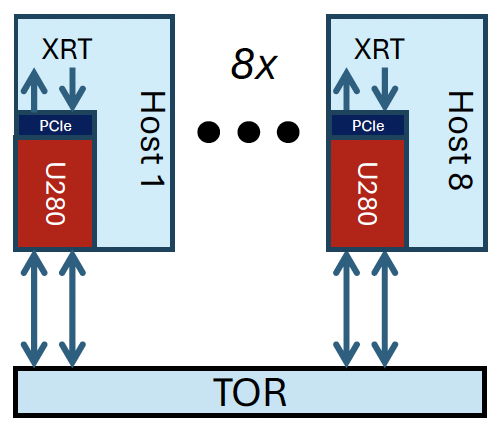
\includegraphics[width=2in]{oct-arch.jpg}
	\caption{Cluster Architecture}
	\label{oct-arch}
\end{figure}

The database was implemented on a cluster of 8 nodes that share a single network switch as shown in figure \ref{oct-arch}. Each node has a Xilinx Alveo U280 PCIe card, containing a XCU280 FPGA and $\SI{8}{\giga\byte}$ of high-bandwidth memory (HBM). Each node is connected to the switch with a $\SI{100}{\giga\bit}$ NIC.

\section{Related Works}

\citeauthor{dlsm} propose a using Log-Structured Merge Trees as a higher-performance alternative to B-trees. However, their system architecture assumes a heterogeneous cluster with some nodes dedicated to memory and other dedicated to processing \cite{dlsm}.

\section{Further Research}

The U280 card contains an entire memory heirarchy that could be leveraged for improved performance using caching. In addition to the $\SI{8}{\giga\byte}$ of HBM used in this experiment, it has $\SI{32}{\giga\byte}$ of slower, off-chip DDR and $\SI{41}{\kilo\byte}$ of faster, on-chip block RAM (BRAM) and UltraRAM.


%%
%% The acknowledgments section is defined using the "acks" environment
%% (and NOT an unnumbered section). This ensures the proper
%% identification of the section in the article metadata, and the
%% consistent spelling of the heading.
\begin{acks}
Acknowledgments go here
\end{acks}


%%
%% The next two lines define the bibliography style to be used, and
%% the bibliography file.
\bibliographystyle{ACM-Reference-Format}
\bibliography{bibfile}


%%
%% If your work has an appendix, this is the place to put it.
../common/appendix.tex


\end{document}
\endinput
%%
%% End of file `sample-sigconf.tex'.
